\documentclass{article}
\usepackage{graphicx}
\begin{document}
	\begin{titlepage}
		\title{Improvements to the immersiveness  of motion controls for video games}
		\date{April 10, 2017}
		\author{T. Maxwell Thomas and David Darrow}
		\maketitle
	\end{titlepage}
	\section{Abstract}
	
	This report details the results of a project to develop an improved motion controller for video games in the form of a glove which translates the hand and arm movements of the user into commands for a connected computer. Described are existing technologies and their shortcomings, technical details of the glove's function, and results of experimental testing of the glove.
	\section{Background}
	
	The problem of improving the immersion of controls is a relatively new one-it was only recently that computational capabilities reached the point where such a project could be undertaken. The games industry has produced several motion control schemes, each with its own shortcomings that the glove is designed to address. More "traditional" motion controls, such as those for the Nintendo Wii, only provide the ability to move the controller as an aide to immersion-the user is still required to press buttons in order to trigger actions. Furthermore, they require that the games they are used for be designed specifically with the controllers in mind-something uncommon in recent games, but impossible for older titles developed before motion controls were released.
	
	Then, there are full-on virtual reality systems such as the HTC Vive. These, while impressive pieces of technology, come with their own set of problems. First off, they require a substantial open area in order to function properly, something not necessarily available to people (consider college students in a cramped dorm room, for example). Furthermore, they're quite expensive, still require button presses-and require support from games in order to be used.
	
	The glove is designed to provide user-customizable controls based on both broad and fine hand and arm movements, with the intention of providing a more natural control input scheme than is afforded by any other input system. Unfortunately, this is unlikely to prove a suitable replacement for existing motion control schemes; the motions take too long for high-precision play, for one thing, and the variety of motions one could reasonably be expected to contend with does not provide sufficient controls for many games. Rather, the glove is intended as a proof-of-concept and novelty item, demonstrating the possibility of such technology. Developing a proper commercial product is beyond the budget and scope of this project, as well as the skills of the authors.
	\section{Design specifics \& potential alternatives}
	
	The glove uses two dedicated 3-axis MMA8451 accelerometers on the thumb and middle fingers, and a 3-axis LSM303 combined accelerometer/magnetometer for reading the glove's current trajectory. Data from the sensors is transmitted ten times per second to a glove-mounted microcontroller over an I\textsuperscript{2}C bus, and then over a serial line transmitting at 9600 baud to the connected computer. Due to the glove's low on-board processing power, and complete lack of long-term storage for anything other than the program, the task of translating glove movements to controls and recording target motions for later use is entirely up to the computer the glove is connected to. 
	
	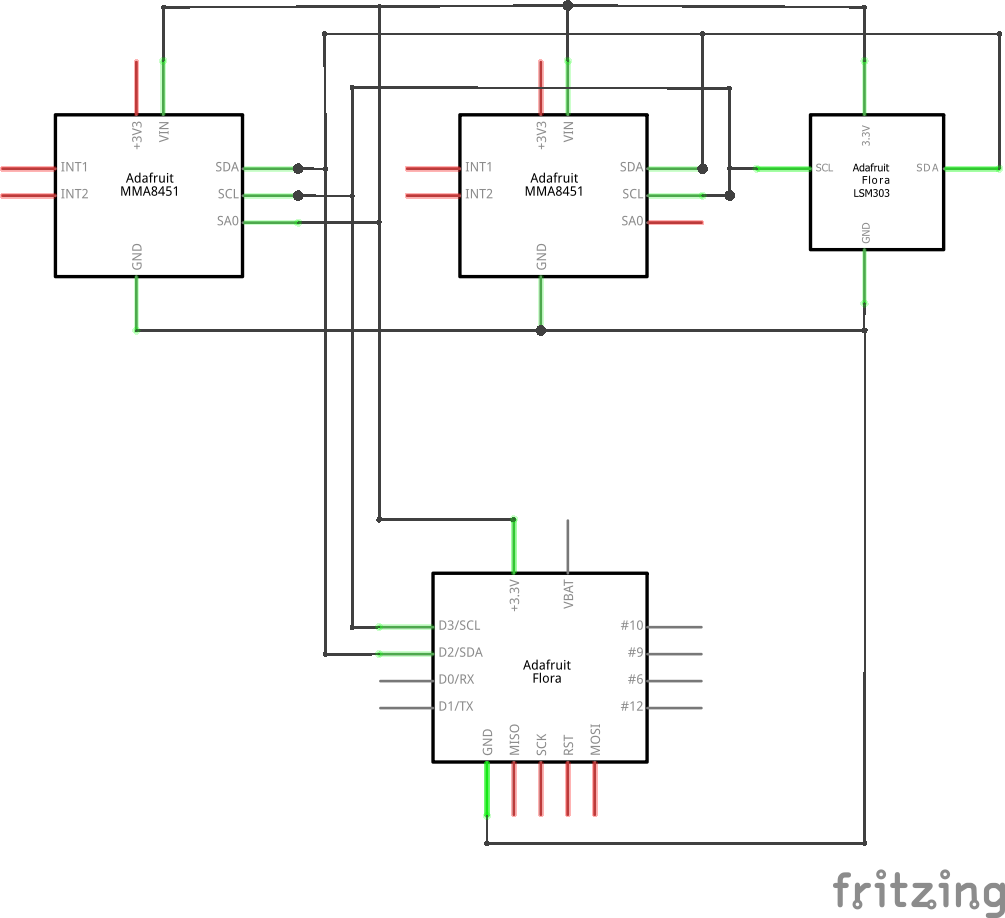
\includegraphics{Glove_schematic}
	
	When recording, the connected computer waits until the acceleration experienced by the glove goes above a specific threshold, and then begins recording the sensor readings, only stopping once acceleration drops below that self-same threshold, indicating cessation of motion. These recorded macros are then stored in a file, for later use. The recording program is run entirely from the terminal, due to both the time it would take to write such an interface, and the agreed-upon lack of necessity for a proper interface for a non-commercial product.
	
	When comparing incoming data to recorded macros (i.e. when the glove is being used as a controller), the glove translates macros from a file as well as incoming data into piecewise, continuously differentiable functions by first expressing the various data points as 12-vectors, and then using cubic splicing to join the vectors into a continuous function. From there, macros or incoming data can be dilated to match in length, and the error between the data and any given macro can be computed as a simple integral. Using interpolation to match the functions is not reasonably possible, due to the even spacing of the data points.
	
	\subsection*{Potential alternatives}
	
	Possible alternatives for the design include using laser position sensors to accurately locate the glove, using a gyroscope instead of a magnetometer for detection of orientation, and using a custom circuit to feed data to the host computer instead of using a microcontroller. Each of these was rejected, for the following reasons:
	
	The laser position sensors, while in every way a more optimal solution to the problem, were well beyond both the means and the skills of the project team to create or use. Furthermore, they would have added additional necessary devices, a suboptimal solution for what was intended to be a standalone device.
	
	A gyroscope would have been less susceptible to interference. However, gyroscopes are subject to drift even over relatively short timeframes, while magnetometers, orienting based on Earth's magnetic field, are not. This is especially true at the commercial level, at which this project is operating. Furthermore, we were able to find an off-the-shelf accelerometer/magnetometer, while no combined accelerometer/gyroscope appeared to be available.
	
	The thought of using a custom chip instead of a microcontroller may have made sense at the commercial level, but for an individual project like this one it was much simpler to just take a microcontroller and program it to do whatever we required of it. Printing circuits is expensive, especially circuits as complicated as would have been necessary, had we tried to make a custom board. Beyond this, though, at a certain point it just makes more sense on every level to use a microcontroller. For starters, they cost pennies to the dollar, and allow for rapid prototyping due to the dynamic nature of the system. Better to just slap one in one's product than go through all the hassle of designing custom electronics that may or may not work on the first go.
	
	
	\section{Results}
	
	
	\section{Conclusion}
	
	
	\section{References \& Bibliography}
	\subsection*{References}
	\subsection*{Bibliography}
\end{document}